\begin{figure}[t]
\centering
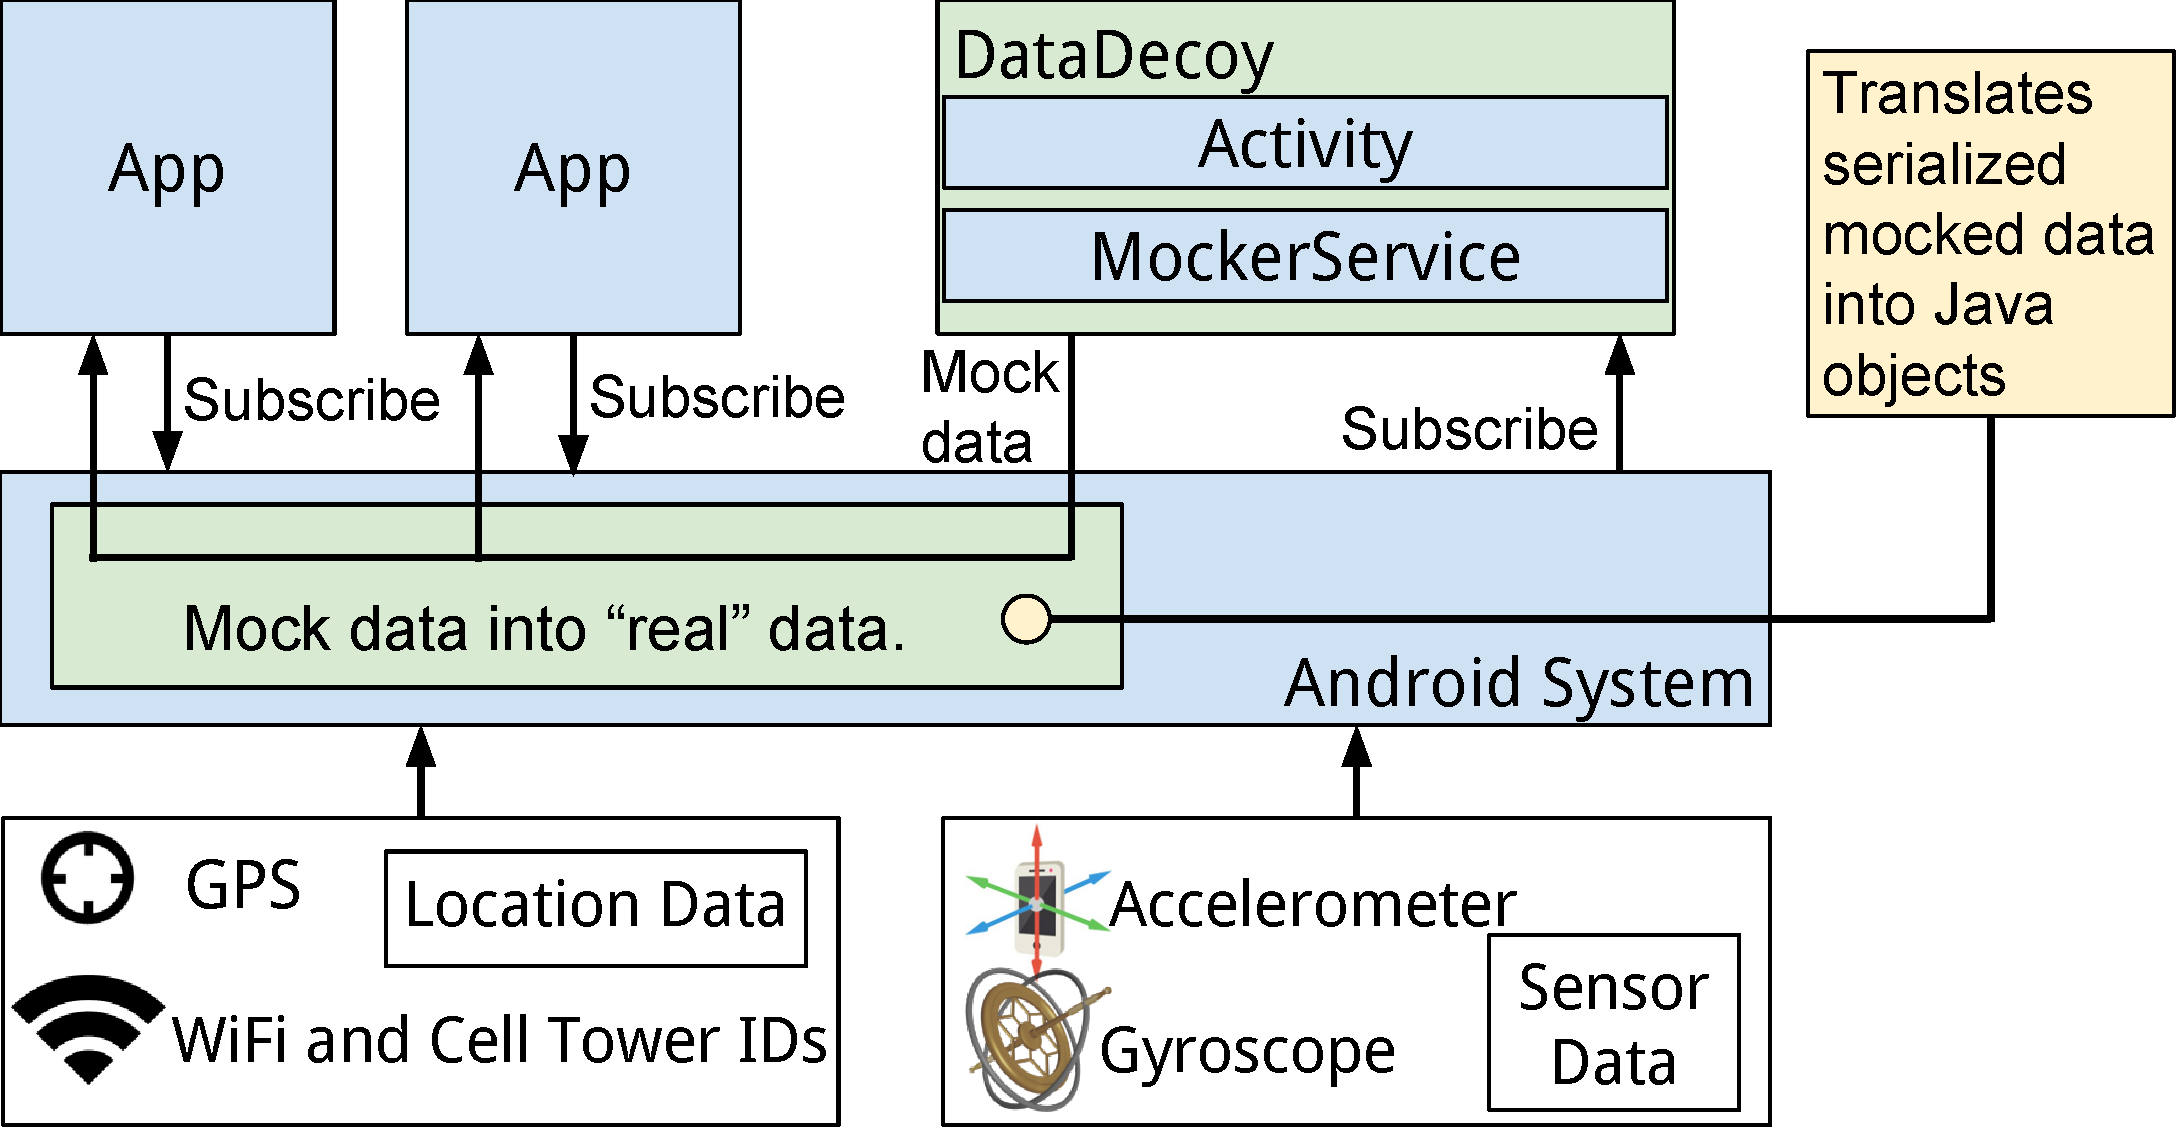
\includegraphics[width=\columnwidth]{./figures/architecture.pdf}

\caption{\textbf{\PocketMocker{} Design.} Details are specific to Android but
would be similar on other platforms.}

\label{fig-design}
\vspace*{-0.2in}
\end{figure}

\section{\PocketMocker{} Design}
\label{sec-design}

This section describes the design of the \PocketMocker{} objective-driven
context mocking system. We begin by developing a set of design requirements
based on the mocking scenarios and taxonomy presented previously, and also
outline the challenges of effective context mocking. We then describe how
\PocketMocker{} uses changes to the smartphone platform and a dedicated app
to perform context mocking.

\subsection{Overview}

We offer the example of Bob from our earlier scenarios as an overview
of how \PocketMocker{}'s components work together to deliver objective-driven
context mocking. \PocketMocker{} consists of two parts:  modifications to the
smartphone platform needed to record and replay mocking traces, and an app
that interacts with the user to record mocking traces and control the mocking
process. Figure~\ref{fig-design} illustrates the interaction between the two
parts of \PocketMocker{}.

Once Bob has formulated his objective---to appear more active to his
smartphone---he is ready to use \PocketMocker{}. The first step is to
determine what activity will accomplish this objective and to record it. In
this case, Bob determines that frequent brisk walks will make him appear more
active. Using the \PocketMocker{} app, he initiates the context recording
process and goes out for a model walk. \PocketMocker{} records every piece of
information it might need later during the mocking process: his GPS location,
the cell towers to which he is connected, visible Wifi access points, and
readings from onboard sensors such as the accelerometer and thermometer---all
appropriately timestamped. Because \PocketMocker{} does not know what apps
will be running during future mocking sessions or what data they will request,
it records as much information as possible even if it is not requested by apps
during the original recording session. This data set comprises the
\textit{mocking trace}.

Once the trace is recorded, Bob can replay it as often as he likes. During the
mocking process, \PocketMocker{} exploits changes to the underlying
smartphone platform to satisfy app requests for real data with time-shifted
false numbers from the mocking trace. While the mocking session is active, the
\PocketMocker{} app displays a notification indicating that mocking is in
progress and how much time remains before it finishes. After completion,
\PocketMocker{} stops returning mocked data and resumes returning real data to
apps.

Based on this use case, we can enumerate several requirements for an
objective-driven context mocking system. First, the user's objective must be
determined and a mocking activity suggested. Second, a mocking trace must be
recorded and linked to the user's objective. Finally, the trace must be
deployed as needed to achieve the user's mocking objective. We describe how
\PocketMocker{} accomplishes these tasks below. We also address how
\PocketMocker{} overcomes two challenges that might allow apps to detect the
mocking process: differences between the mocking trace and the real current
context, and spatial discontinuities. Time-shift mocking has somewhat
different requirements, and we discuss them separately at the end of this
section.

\subsubsection{Linking mocking traces and objectives}

To begin, \PocketMocker{} must be able to link mocking traces with
user-defined objectives, so that it knows what trace will achieve each
objective. In Bob's example, \PocketMocker{} must be able to associate the
trace of Bob taking a walk with Bob's desire to appear more active. This
process has both a qualitative and quantitative component. Qualitatively,
\PocketMocker{} may suggest activities that would naturally be linked with a
specific objective. If Bob wants to be more active, he should take a walk. If
Alice wants to appear more healthy, she should eat at a healthy
restaurant---and not eat at the fast-food restaurant. \PocketMocker{}'s app
provides a library of objectives (''appear more fit'') and associated
suggestions for mocking traces (''take a walk''). We also expect users will
be well-served by their own intuition.

\subsubsection{Collecting, storing, and replaying traces}

Second, \PocketMocker{} must be able to collect, store and replay mocking
traces. Trace collection is currently initiated by the \PocketMocker{} app and
performed entirely at the app level. To ensure that during mocking
\PocketMocker{} can return data from any source consistent with the mocked
context, \PocketMocker{} currently enables all sensors that could provide
relevant information and samples them aggressively, storing timestamped data in
a set of local databases. As one optimization to the process of recording
mocking traces, \PocketMocker{} uses changes to the users current location to
trigger the immediate collection of location-specific data. For example, when
\PocketMocker{} detects a location change it immediately stores new Wifi scan
results and cellular signal strength information. As long as the user is not
moving, these kinds of data are sampled more slowly.

Unlike trace collection, mocking trace replay requires platform support.
\PocketMocker{} modifies the underlying smartphone platform to add an
interface allowing it to inject mocked data. Once the user begins replaying
the trace, \PocketMocker{} reads data from all sensor databases associated
with the trace and uses this new interface to inject it into the platform.
Any app requests for data contained in the mocking then return mocked data.

\subsubsection{Initiating mocking sessions}

Third, \PocketMocker{}'s app helps the user remember to initiate mocking
sessions. Each recorded trace can be annotated with a frequency which
\PocketMocker{} uses to help prompt the user to deploy the trace. For
example, Bob may want to go for a walk once every day, and by annotating the
trace with his goal \PocketMocker{} knows when to provide reminders.

\subsection{Consistency Challenges}

A significant challenge when mocking is addressing differences between the
mocking context and the real context to ensure that mocking proceeds
consistently. At present \PocketMocker{} does not attempt to fully defend the
mocking context from suspicious apps---we leave that challenge as future
work. However, \PocketMocker{} still attempts to ensure that the mocking
context is consistent and does not create obvious problems or physical
impossibilities that could either break app functionality or send an
unmistakable signal that something unusual is happening. First, we look at
how \PocketMocker{} masks differences between the mocking context and the
real context. Second, we address spatial continuity, a specific consistency
problem facing the \PocketMocker{} system.

\subsubsection{Differences with the mocking context}

Here we examine specific differences between the mocking context and the real
context and address how \PocketMocker{} deals with each case:

\begin{itemize}

\item \textbf{Location:} \uline{the phone is one place in the mocking context
and another location in the real context.} To ensure location consistency,
\PocketMocker{} collects all data associated with the mocked location. During
the mocking session an app will not only have the mocked location coordinates
returned, but will also see the same Wifi access points and be connected to
the same cell tower with the same signal strength as it would at the mocked
location.

\item \textbf{Device configuration:} \uline{the accelerometer was not used
during the mocking context but is enabled by an app in the real context.}
Here \PocketMocker{} exploits the fact that it records all information about
the smartphone while recording the mocking trace, meaning that it can handle
requests to use any device feature during replay.

\item \textbf{Connectivity:} \uline{the phone was connected during the
mocking context but there is a different or no network connection available
in the real context.} There are two cases to consider here. If the smartphone
has any connection in the real context, \PocketMocker{} will allow apps to
use that connection but return mocked connection \textit{attributes}. So if
the connection is actually over a Wifi network but only a 3G mobile data
network is available, \PocketMocker{} will establish connections over the
available network but tell apps that they are connected over the mocked Wifi
network. At present \PocketMocker{} makes no attempt to alter connection
properties such as latency or bandwidth of the real connection to match the
mocked connection, and in some cases this is not possible. We leave dealing
with attempts by suspicious apps to use these properties to pierce the
mocking context as future work.

A more difficult problem is providing a mocked connection when no real
connection exists. Since this is impossible, \PocketMocker{} simply
synchronizes this aspect of the mocking context with the real context and
does not provide any mocked networking information while a real network is
unavailable. While this creates variance in the mocking context, networks
naturally go up and down and a user may have disabled the phone networking
manually, meaning that lack of networking connectivity at a location where it
is typically available cannot necessarily be interpreted by an app to mean
that mocking is happening. Smartphone apps have to naturally handle this kind
of variation in networking conditions due to mobility and changes in user
configuration.

\end{itemize}

It is also important to point out things that \PocketMocker{} \textit{does
not mock}, including user interaction, battery level, and the microphone
readings. While mocking user interaction may be necessary to mislead certain
types of apps, it is not necessary to mock the apps that \PocketMocker{}
currently targets that collect and interpret data collected passively. More
importantly, replaying interaction would prevent the user from using their
smartphone while mocking was active.

Replaying microphone readings represent a similar challenge since the
microphone is used by the phone feature of the smartphone which we expect
that users will not want to disable during mocking. Unfortunately, not
replaying certain aspects of the audio environment may allow other apps to
detect a different between the mocked context and the real context, such as a
user claiming to be at a loud bar but actually still at their quiet home. We
are planning to address this current limitation of \PocketMocker{} in the
future, either by providing a pass-through for real context audio to apps
where it represents input, or by merging audio recorded during replay with
the audio from the mocking trace.

Finally, if replayed battery levels would represent another continuity
challenge similar to the spatial continuity challenge presented next. If
\PocketMocker{} produced mocked battery readings during trace replay that
represented the actual rate of battery usage during the trace, the system
would be left with a discontinuity when the trace completed as the battery
level would either have to abruptly increase or decrease to merge with the
actual battery level. On the other hand, continuing to report actual battery
levels during trace poses no threat to the mocking context and is actually
more realistic, since the battery level will continue to track app usage of
the device. For example, if the mocking trace was performed while no apps
were rapidly using energy, and then apps did perform activities that led to
heavy energy usage during replay, replaying the original battery drain would
allow an observant app to identify a difference between the mocking and real
contexts. Continuing to report actual battery levels is both easier and more
correct.

\subsubsection{Ensuring spatial continuity}

Given that smartphones can and do track their users location, and that this
information reveals a great deal about their lives, \PocketMocker{} is
designed to allow mocking location and user movement. However, this creates a
continuity challenge when the mocking trace ends at a different place from
the user's current location. We discuss in Section~\ref{sec-future} how
future version of \PocketMocker{} will use user-generated mocking libraries
to be able to synthesize mocking traces linking any two points where the user
has previously been, but our current prototype has no good way to address
this problem. And while we are currently focusing on mocking unsuspecting
apps and not addressing all attacks apps could perform on the mocking
context, sudden changes in location are both an all-too-obvious indication of
mocking and might also cause some apps to malfunction.

Currently, \PocketMocker{} works around this challenge by interacting with the
user. While a mocking trace is being replayed, a notification is displayed
informing the user of the time left before the mocking process completes and
the distance from the user to the location where the trace ends. Once the
trace ends, if the user's location is close to where the trace completes
\PocketMocker{} will simply allow the trace to end normally and merge the
real and mocking context. If the user is not close to where the trace
completes, \PocketMocker{} generates an notification asking the user to
either reach the correct location or allow the spatial discontinuity. Until
the user responds to the dialog or reaches the required location,
\PocketMocker{} continues to mock them at the mocking traces final location,
using the lingering capability described next. This also allows
\PocketMocker{} to perform backward time shifting on an existing trace. In
Jerry's example, when it is time to return home he initiates a pre-recorded
trace of his return. Once his trace reaches home, it will linger there until
he arrives at some later time.

\subsection{Lingering}

In addition to the record-and-replay functionality we have already described,
\PocketMocker{} also supports \textit{lingering}. Lingering is a mocking
primitive that can be used in several ways: to time-extend a mocking trace,
to conceal an undesirable activity, or to perform time-shift mocking. In the
scenarios described earlier both Alice, Jerry, and Carol's mocking activities
require this capability. Carol uses lingering to conceal her coffee break,
Jerry uses it to time-shift his return home, and Alice uses it to time-extend
her visit to the healthy restaurant to match the time she spends eating fast
food.

To linger, \PocketMocker{} records a small amount of context at a particular
location and then replays it repeatedly. To make the data delivered to apps
during the lingering process more realistic, and prevent apps from detecting
the mocking process by observing repeated readings, \PocketMocker{} injects
noise into the data returned during the lingering session, performing small
changes to the reported location, sensor readings, Wifi scan results, and
network signal strengths.

To time-extend a trace, the app allows users to indicate linger points during
trace recording. During replay, once the trace reaches a linger point
\PocketMocker{} will linger until instructed to proceed by the user. Once
Alice is ready to leave the fast-food restaurant, she tells \PocketMocker{}
to proceed past the linger point she inserted into her trace of visiting the
healthy restaurant. To conceal an undesirable activity, the \PocketMocker{}
app allows lingering to be initiated at any time. A small amount of context
is recorded and then replayed until the lingering session is canceled. So
Carol can initiate the lingering session at work, and then bring her phone
with her to her coffee break while appearing to remain at work.

Forward-shifting a trace is a three-step process. First, \PocketMocker{}
collects a small amount of context at the current location in order to linger
and begins the lingering process. Second, \PocketMocker{} records a user
moving to a new location while continuing to return lingering data. Finally,
once the user is ready to merge their real and mocked context,
\PocketMocker{} stops lingering and begins replaying the transition trace
until the user reaches their current location.
